% Chapter 6
%
\chapter{Experiments} % Main chapter title
%
\label{Chapter6} % For referencing the chapter elsewhere, use \ref{Chapter4} 
%
In this chapter the experiments conducted will be discussed. The reasoning behind doing them, the way they were conducted, as well as the results, will be explained. The impact of the results and what the results mean for the usage of SendIt will also be clearly stated and evaluated.
%
\section{Motivation and contribution}
%
The original goal of doing these experiments was to evaluate the time limit for successfully establishing a connection, in regards to the WebRTC Offer and Answer exchange (from now on referred to as the connection setup). The Serverless mode requires manual interactions from the users, so knowing the time constraint is important for using the system optimally. In addition, if improvements were to be implemented, it would be necessary to have a benchmark to test against. It would also give a good indication on how to best proceed with improving the solution. As an added bonus, the setup for the experiments can also function as a framework for testing possible improvements and enhancements to the system.

The motivation for doing these experiments was to test the lifetime of the connection setup. Based on the results, the usability and limitations of the Serverless mode would be clear. This indicates the advantages and limitations of the Serverless mode, which allows for better decision-making when choosing modes. It also allows for a clear definition of the potential problems with the serverless solution and gives a tangible, concrete frame of reference for improving the solution.
In more detail, the goal of the experiments can be divided into four parts:
%
\begin{itemize}
	\item Find the approximate lifetime of the Offer
	\item Find the approximate lifetime of the Answer
	\item Find the approximate lifetime of the connection setup
	\item Find the most impactful part of the connection setup
\end{itemize}
%
Since the experiments are meant as a reference and benchmark for SendIt's functionality, the setup mimics SendIt's connection setup and exchange as much as possible. This means the results of the experiments should be directly transferable to SendIt and the results should reflect what to expect from SendIt's current functionality. The results are also similar to the conditions and results experienced when developing and testing SendIt.
%
%
\begin{figure}[th]
  \centering
  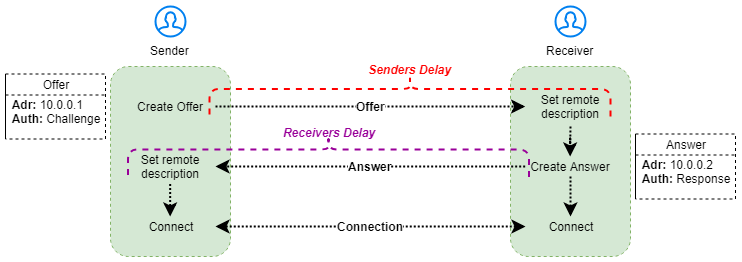
\includegraphics[width=\textwidth]{Figures/Terms}
  \decoRule
  \caption[Experiment terminology]{Simplified illustration of experiment setup}
  \label{fig:terms}
\end{figure}
%
\section{Terminology}
%
The terminology is as follows:\\
{\bfseries Offer:} WebRTC connection offer generated by the Sender in order to initiate a connection with the receiver.\\
{\bfseries Answer:} WebRTC connection answer generated by the Receiver, from the Offer received, to complete the connection setup.\\
{\bfseries Sender's delay} (\textit{S}){\bfseries :} is the delay from creation of the Offer until it is received by the other endpoint.\\
{\bfseries Receiver's delay} (\textit{R}){\bfseries :} is the delay from creation of the Answer until it is received by the other endpoint.\\
{\bfseries Split delay:} is the delay split equally between \textit{S} and \textit{R}. If the delay is 10 seconds, it means 5 seconds Sender's delay and 5 seconds Receiver's delay, for a total of 10 seconds delay.
For a better understanding of these terms, look at the simplified representation in \Cref{fig:terms}.
%
\section{Implementation and results}
%
In these experiments, the success-rate of connections between a server and a client was measured. The connection was created using WebRTC with a varying delay before the Offer and/or Answer was shared. The experiments were conducted by having users connect to a web server over HTTP and naturally having the server deliver content via HTTP. After the necessary HTML and JavaScript had been delivered to the client, they would try to establish another connection to the server using WebSockets. This allows for bi-directional and efficient communication. 
Over this WebSocket connection, the connection setup for the following tests was done. The P2P connection and setup was done utilizing the WebRTC PeerConnection functionality. The whole experiment consisted of three test sets:
%
\begin{itemize}
	\item Test set 1 - Sender's delay (\textit{S})
	\item Test set 2 - Receiver's delay (\textit{R})
	\item Test set 3 - Split delay
\end{itemize}
%
Each of these test sets consisted of five tests. Once all test sets were finished (or when the client disconnected), the client shared their log with the server, and the server stored both logs for analysis and comparison. The pattern described below indicates how one test was done. Once this had been completed for all five tests in all three test sets (for a total of 15 tests), the experiment was considered finished, and the connection torn down. If a client disconnected before finishing all tests, the results for the tests completed up until that point was shared with the server, and stored.

The tests were done as follows:
For each test, the respective WebRTC Offer and Answer was exchanged. Depending on the test case, the sharing of the Offer or the Answer, or both, was delayed by varying length. Once the exchange had completed, the server and the client tried to establish a WebRTC P2P connection. Once this was done, a status check was immediately issued in order to check the result of the connection establishment. The results of this status check was used to indicate whether the connection was successful or not.

It is important to note that in initial tests, the results of the status check was noted before trying to utilize the P2P channel to do actual data transfers. In these tests, the result of the status check always correctly indicated whether the connection was successful or not. As such this status check was considered sufficient to indicate the result of the connection establishment. The result of the check was then logged for both server- and client-side. The P2P connection was then torn down and a new connection setup began.
%

For the illustrations in the following sections, the percentage of successful P2P connections is represented on the vertical axis, and the total delay before trying to establish the P2P connection on the horizontal axis. Each test set has a different type of line. 
%
%
\subsection{Experiment 1}
%
\begin{figure}[th]
  \centering
  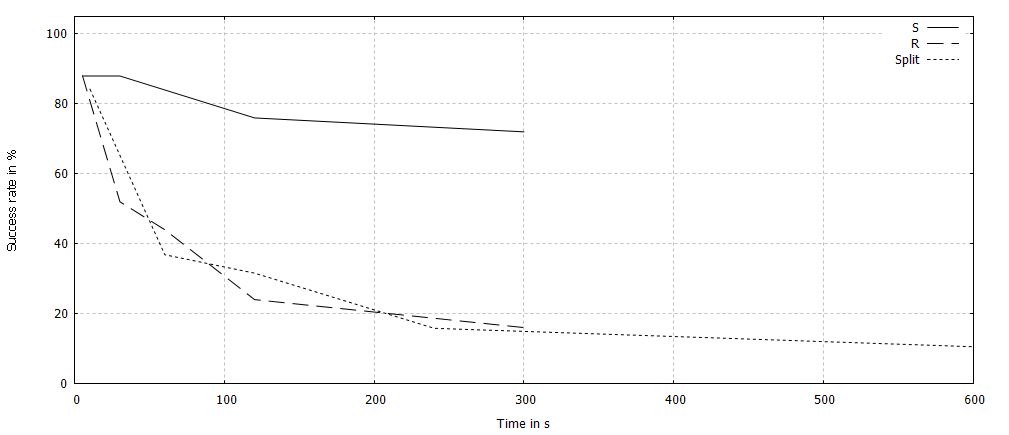
\includegraphics[width=\textwidth]{Figures/Exp1_res}
  \decoRule
  \caption[Results Experiment 1]{Delayed WebRTC connection setup success rate with Server as Sender (\textit{S})}
  \label{fig:exp1}
\end{figure}
%
The results of the first experiment are shown in \Cref{fig:exp1} The server took the role of Sender in all connections in this experiment.

The size of the dataset is as follows: test sets 1 and 2 (\textit{S} \& \textit{R}) consists of 25 connections. For test set 3 (Split delay), only 19 connections completed all tests. This is after cleaning the dataset. Connections that failed all tests were removed because the probability of failing all tests and still being a supported connection is very low. These connections are assumed not to be in the target group of computers eligible to use SendIt, and as such would skew the results.

Now lets discuss the findings and implications of this experiment (See \Cref{fig:exp1}). As you can see, \textit{S} is fairly irrelevant. Even at 300 seconds (5 minutes) the success rate is 72\%. \textit{R} is much more important. At a 5 seconds delay, \textit{S} and \textit{R} have the same success rate. However, at 30 seconds, there is a gap of 36\% (\textit{S}=88\%, \textit{R}=52\%). This indicates that the problem with keeping a connection open largely resides on the Receiver's end. Splitting the delay equally between \textit{S} and \textit{R} (as indicated by 'Split Delay'), seem to improve connectivity compared to \textit{S}, which corroborates the theory that \textit{S} has more influence on the success rate of creating a connection.

One factor that might influence this result is that, in this experiment, the test-server always acted as \textit{S}. The server may have a more stable internet-connection than most endpoints. As such, another experiment was conducted where the server acts as \textit{R}, so the results could be compared and the conclusion re-evaluated.
%
%
\subsection{Experiment 2}
%
\begin{figure}[th]
  \centering
  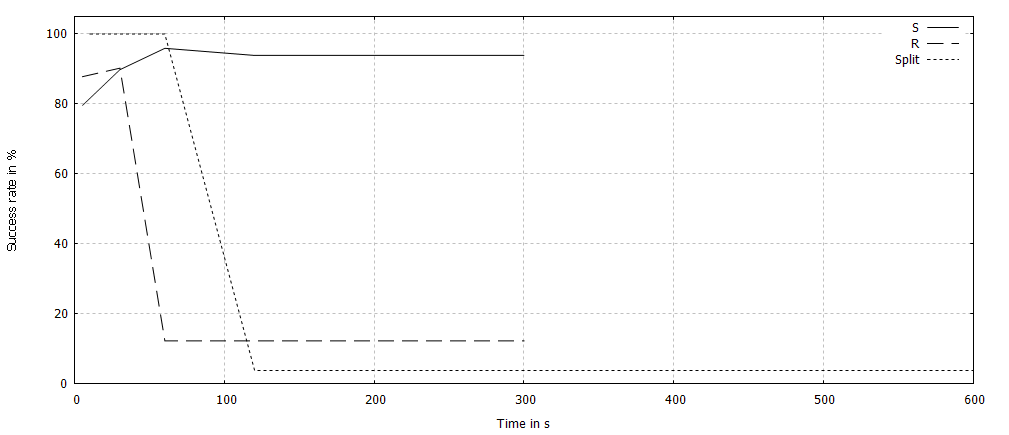
\includegraphics[width=\textwidth]{Figures/Exp2_res}
  \decoRule
  \caption[Results Experiment 2]{Delayed WebRTC connection setup success rate with Server as Receiver (\textit{R})}
  \label{fig:exp2}
\end{figure}
%
The results of the second experiment are shown in \Cref{fig:exp2}. The server took the role of Receiver in all connections in this experiment.

The size of the dataset is as follows: test set 1 (\textit{S}) consists of 49 connections. Test set 2 (\textit{R}) has 41 connections. Finally, for test set 3 (Split delay), there are 27 connections. This is after cleaning the dataset. Connections that failed all tests were removed because the probability of failing all tests and still being a supported connection is very low. These connections are assumed not to be in the target group of computers eligible to use SendIt, and as such would skew the results.

Because of some technical issues during the second experiment, a lot of connections timed out after only completed a few tests. As such, connections who did not complete the first test set (\textit{S}) were also excluded. During analysis of the results, it also became clear that there were a number of repeating connections from the same client, with identical results, in a very short time span. As such, results from the same IP with identical results, with less than one hour between tests, were removed. This resulted in a more correct representation of the data gathered.

Now lets discuss the findings and implications of this experiment (See \Cref{fig:exp2}). In a similar fashion as in Experiment 1, \textit{S} is much less impactful than \textit{R}. In this experiment, \textit{R} has an even more drastic and rapid decrease in success-rate. Already after 60 seconds, the rate has dropped to only 12\%. \textit{S} on the other hand, experiences very little variation in success-rate over time. It is safe to say that this experiment indicates that \textit{S} is insignificant in comparison to \textit{R}. It is also interesting to note that the Split delay has an even more severe drop-off than \textit{R}. Between 60 and 120 seconds, it drops from 100\% success-rate to only 4\%. Why this is the case is hard to evaluate, as there is no clear indication why this behavior occurs. 
%
%
\section{Impact and findings}
%
\begin{figure}[th]
  \centering
  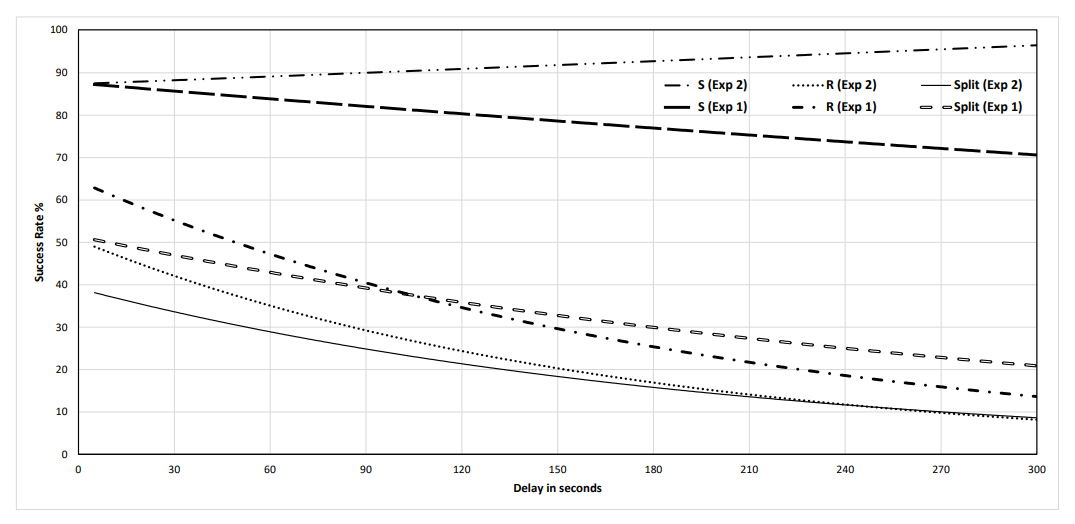
\includegraphics[width=\textwidth]{Figures/Experiment_comp}
  \decoRule
  \caption[Experiment comparison]{Shows the exponential approximation of the results in the two experiments for comparison. These indicate how the average results will look over time.}
  \label{fig:expcomp}
\end{figure}
%
\begin{table}
	\caption[Comparison of Sender's delay]{Comparison of the Sender's delay in Experiments 1 and 2. The values represent the rate of success in establishing a connection.}
	\label{tab:comp_send}
	\centering
	\begin{tabular}{c@{\qquad}ccccc}
	    \multirow{3}{*}{\raisebox{-\heavyrulewidth}{\textit{S}}} & \multicolumn{5}{c}{Time in seconds}\\
	  	\cmidrule{2-6}
        & 5 & 30 & 60 & 120 & 300\\
        \midrule
        $Experiment~1$ & 88\% & 88\% & 84\% & 76\% & 72\% \\
        $Experiment~2$ & 80\% & 90\% & 96\% & 94\% & 94\% \\
        \bottomrule
	\end{tabular}\\
\end{table}
%
\begin{table}
	\caption[Comparison of Receiver's delay]{Comparison of the Receiver's delay in Experiments 1 and 2. The values represent the rate of success in establishing a connection.}
	\label{tab:comp_recv}
	\centering
	\begin{tabular}{c@{\qquad}ccccc}
		\multirow{3}{*}{\raisebox{-\heavyrulewidth}{\textit{R}}} & \multicolumn{5}{c}{Time in seconds}\\
	  	\cmidrule{2-6}
        & 5 & 30 & 60 & 120 & 300\\
        \midrule
        $Experiment~1$ & 88\% & 52\% & 44\% & 24\% & 16\% \\
        $Experiment~2$ & 90\% & 93\% & 12\% & 12\% & 12\% \\
        \bottomrule
	\end{tabular}\\
\end{table}
%
\begin{table}
	\caption[Comparison of Split delay]{Comparison of the Split delay in Experiments 1 and 2. The values represent the rate of success in establishing a connection.}
	\label{tab:comp_split}
	\centering
	\begin{tabular}{c@{\qquad}ccccc}
      	\multirow{3}{*}{\raisebox{-\heavyrulewidth}{Split~delay}} & \multicolumn{5}{c}{Time in seconds}\\
	  	\cmidrule{2-6}
        & 10 & 60 & 120 & 300 & 600\\
        \midrule
        $Experiment~1$ & \textasciitilde88\% & \textasciitilde37\% & \textasciitilde32\% & \textasciitilde16\% & \textasciitilde11\% \\
        $Experiment~2$ & 100\% & 100\% & \textasciitilde4\% & \textasciitilde4\% & \textasciitilde4\% \\
        \bottomrule
	\end{tabular}\\
\end{table}
%
The results from these experiments can now be compared (Shown in \Cref{tab:comp_send}, \Cref{tab:comp_recv}, \Cref{tab:comp_split} and \Cref{fig:expcomp}), by examining the collected data.

As you can see, the results are fairly similar. This indicates that delaying the Answer has far more impact than delaying the Offer. One can assume this by comparing the success-rate of connections for \textit{R} and \textit{S} in \Cref{tab:comp_send} and \Cref{tab:comp_recv}. The percentages drop drastically, as the delay increases for \textit{R}. On the contrary, \textit{S} has only a slight decrease in success-rate (and only for Experiment 1). From this one can conclude that the original assumption was correct: The Answer is by far the most impactful part of the connection setup.

By looking at and comparing the results from Experiments 1 and 2, one can clearly identify that \textit{R} experiences a significant drop when the delay is between 30 and 60 seconds. With a success-rate of respectively 52\% and 93\% for 30 second delay, compared to 44\% and 12\% for a 60 second delay. With this knowledge, one can conclude that the average lifetime of \textit{R} is somewhere between these two values.

One can also draw the conclusion that the Offer can last at least 5 minutes, based on the experiments. The lowest success-rate for the Offer was 72\% at 300 seconds (5 minutes) delay, in Experiment 1. For Experiment 2, this value was comparatively 94\%. From this it can be extrapolated that it is likely that a connection will be successful, even if \textit{S} approaches, or even extends past 5 minutes.

By combining the results of two previous conclusions: \textit{S} having a lifetime of at least 5 minutes, and \textit{R} having a lifetime between 30 and 60 seconds, the average lifetime of the connection setup can be found. Even though \textit{R} experiences a rapid decrease between 30-60 seconds, \textit{S} seems to have the ability to extend past 5 minutes. For this reason, the lifetime of the connection setup will be around 6 minutes. This should be kept in mind if one is utilizing the Serverless mode.

Finally, an interesting observation, however expected, is that when the Server acted as the Receiver (Experiment 2), the results were far more volatile, then when the roles were reversed (Experiment 1). This is probably because it is beneficial to have the most stable endpoint initiate the connection, as it allows for more predictable results.

The more stable connection is likely to have more routes to be reached through, and as such, is more likely to result in a more stable setup environment. If the route changes, with the more stable endpoint being the initiator, one of the other routes can be used instead. This is not the case for unstable, constantly changing endpoints, as they may only have one route, or the other routes also become unusable. It should be emphasized that there is no proof to back up such an assumption in these experiments, but it seems to be the likely scenario.
%
